\documentclass{article}
\usepackage{fullpage}
\usepackage{multicol,multirow}
\usepackage{tabularx}
\usepackage{ulem}
\usepackage[utf8]{inputenc}
\usepackage[russian]{babel}
\usepackage{pgfplots}
\usepackage{graphicx}

\begin{document}

\section*{Лабораторная работа №7 по курсу «Численные методы»}

Выполнил студент группы М8О-408Б-20 Попов Матвей.
\\
Преподаватель: Пивоваров Д.\,Е.

\subsection*{Цель}

Решить краевую задачу для дифференциального уравнения эллиптического типа. 
Аппроксимацию уравнения произвести с использованием центрально-разностной 
схемы. Для решения дискретного аналога применить следующие методы: метод 
простых итераций (метод Либмана), метод Зейделя, метод простых итераций с 
верхней релаксацией. Вычислить погрешность численного решения путем сравнения 
результатов с приведенным в задании аналитическим решением $ U(x, y) $. 
Исследовать зависимость погрешности от сеточных параметров $ h_x, h_y $.

\subsection*{Вариант 1}
$$ \frac{\partial^2 u}{\partial x^2} + \frac{\partial^2 u}{\partial y^2} = 0 $$
$$ u(0, y) = y $$
$$ u(1, y) = 1 + y $$
$$ u(x, 0) = x $$
$$ u(x, 1) = 1 + x $$
Аналитическое решение: $$ U(x, y) = x + y $$

\subsection*{О программе}
Модуль для вычислений написан на Go 1.21, модуль для визуализации написан 
на Python с использованием Jypiter Notebook. Реализации всех методов находятся 
в папке internal.

\subsection*{Инструкция к запуску}
Для запуска должны быть установлены Go 1.21 и Python 3, а также модули numpy и 
matplotlib. Для получения результатов и их визуализации достаточно запустить 
все ячейки в lab07.ipynb.

\subsection*{Результаты}
\begin{center}
Полученные вычисления на момент времени $ t = 0.5 $
\\
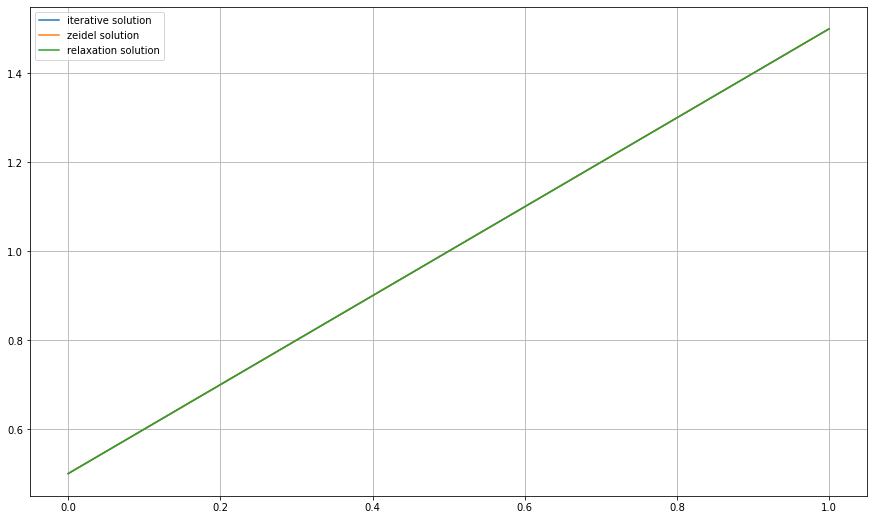
\includegraphics[scale=0.25]{img/img01.png}
\pagebreak
\\
Изменение погрешности
\\
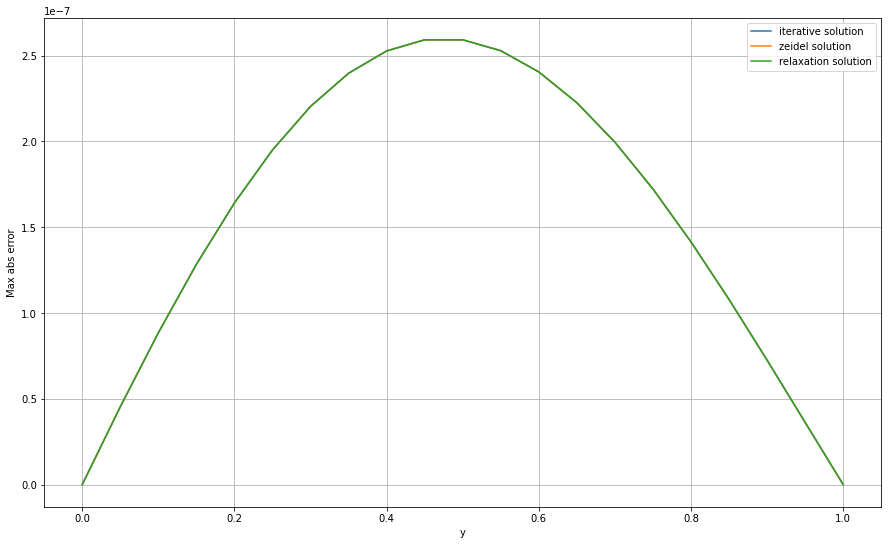
\includegraphics[scale=0.25]{img/img02.png}
\end{center}

\subsection*{Вывод}
Проделав лабораторную работу, я решил начально-краевую задачу для ДУ 
эллиптического типа, используя три различных метода решения СЛАУ, и проверил 
погрешности полученных вычислений.

\end{document}
